\begin{flushright} {\tiny {\color{gray} pair\_p1ppp10.tex}} \end{flushright}
%~~~~~~~~~~~~~~~~~~~~~~~~~~~~~~~~~~~~~~~~~~~~~~~~~~~~~~~~~~~~~~~~~~~~~~~~~~~~~~~~~~~~~~~~~~~~~~~~~~


\begin{center}
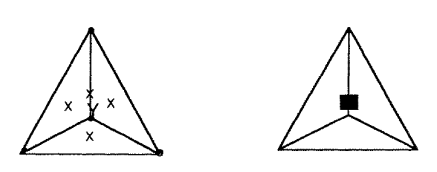
\includegraphics[width=6cm]{images/pair_p1ppp1/p1ppp1}\\
{\captionfont Taken from \textcite{begt92} (1992).}
\end{center}

In Table I of \textcite{begt92} (1992) we find:
\begin{eqnarray}
\bN_1(r,s,t) &=& (1-r-s-t)-\frac13 (\bN_5+\bN_6+\bN_7)-\frac14 \bN_9 \qquad \vec{r}_1=(0,0,0) \nn\\
\bN_2(r,s,t) &=& r-\frac13 (\bN_5+\bN_6+\bN_8)-\frac14 \bN_9 \qquad \vec{r}_2=(1,0,0) \nn\\
\bN_3(r,s,t) &=& s-\frac13 (\bN_5+\bN_7+\bN_8)-\frac14 \bN_9 \qquad \vec{r}_3=(0,1,0) \nn\\
\bN_4(r,s,t) &=& t-\frac13 (\bN_6+\bN_7+\bN_8)-\frac14 \bN_9 \qquad \vec{r}_4=(0,0,1) \nn\\
\bN_5(r,s,t) &=& 27(1-r-s-t)rs-\frac{108}{256}\bN_9          \qquad \vec{r}_5=(\frac13,\frac13,0) \nn\\
\bN_6(r,s,t) &=& 27(1-r-s-t)rt-\frac{108}{256}\bN_9          \qquad \vec{r}_6=(\frac13,0,\frac13) \nn\\
\bN_7(r,s,t) &=& 27(1-r-s-t)st-\frac{108}{256}\bN_9          \qquad \vec{r}_7=(0,\frac13,\frac13) \nn\\
\bN_8(r,s,t) &=& 27rst-\frac{108}{256}\bN_9  \qquad\qquad\qquad\quad \vec{r}_8=(\frac13,\frac13,\frac13)\nn\\ 
\bN_9(r,s,t) &=& 256(1-r-s-t)rst \qquad\qquad\qquad \vec{r}_9=(\frac14,\frac14,\frac14)\nn
\end{eqnarray}
Note that we can verify that
\begin{eqnarray}
\sum_{i=1}^8 \bN_i(r,s,t) 
&=& \bN_1 +\bN_2 +\bN_3 +\bN_4 +\bN_5 +\bN_6 +\bN_7 +\bN_8 +\bN_9\nn\\
&=& (1-r-s-t)-\frac13 (\bN_5+\bN_6+\bN_7)-\frac14 \bN_9 \nn\\
&+& r-\frac13 (\bN_5+\bN_6+\bN_8)-\frac14 \bN_9 \nn\\
&+& s-\frac13 (\bN_5+\bN_7+\bN_8)-\frac14 \bN_9 \nn\\
&+& t-\frac13 (\bN_6+\bN_7+\bN_8)-\frac14 \bN_9 \nn\\
&+& +\bN_5 +\bN_6 +\bN_7 +\bN_8 +\bN_9 \nn\\
&=& 1 
+ (-\frac13-\frac13-\frac13 + )  \bN_5
+ (-\frac13-\frac13-\frac13 + )  \bN_6 \nn\\
&& + (-\frac13-\frac13-\frac13 + )  \bN_7
+ (-\frac13-\frac13-\frac13 + )  \bN_8 
+ (-\frac14 -\frac14-\frac14 -\frac14 +1) \bN_9 \nn\\
&=& 1
\end{eqnarray}



